\chapter{Systementwurf}
%Bildgewinnung
\section{Erzeugen von Sensoroutput}
%
\subsection{Kameradaten}
\begin{figure}[h!]
  \begin{center}
    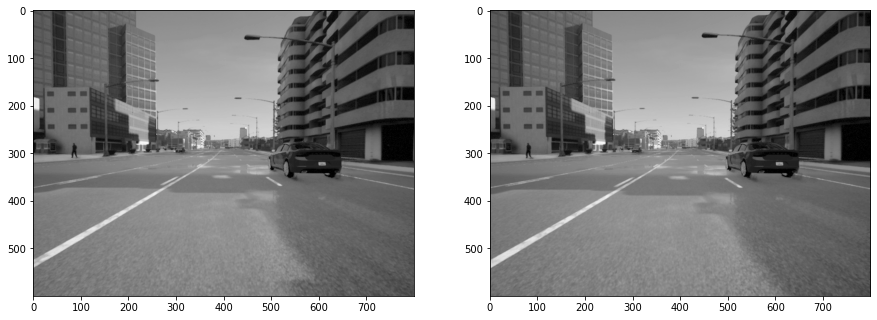
\includegraphics[width=\textwidth]{pictures/load_images_systementwurf.png}
    \caption[Eingansdaten Bilder aus Stereoaufbau in CARLA Simulator]{Grayscale konvertierte RGB Bilder aus Stereo Setup auf Fahrzeug in CARLA Simulator montiert.}
  \end{center}
\end{figure}
%
Alle Sensoroutputs werden im Simulator generiert. 

Zu Beginn kommen Kameradaten in das System. Entweder in Form von zwei RGB Bildern, die um eine Baseline $b=50 cm$ verschoben aufgenommen wurden. 
%
Oder als RGB und Depth Image Paar.

\subsection{Node für Kamerasynchronisation}
\begin{center}
  \begin{figure}[h!]
    \centering
    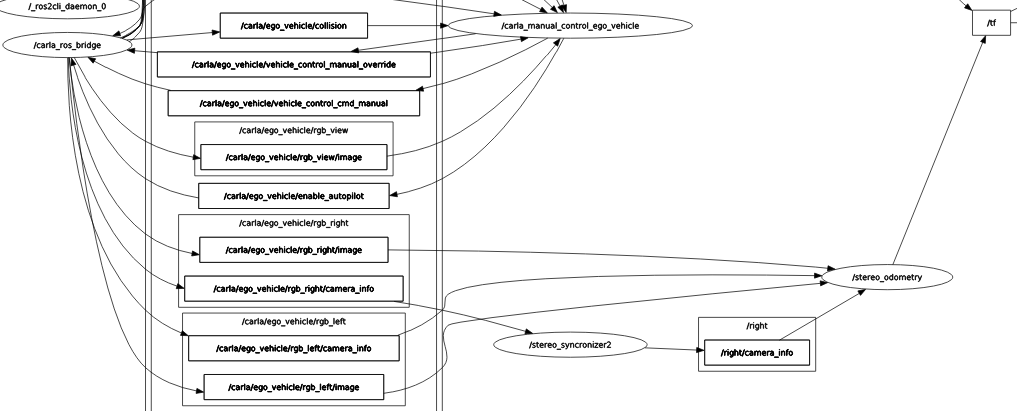
\includegraphics[width=\textwidth]{pictures/06_ros_topic_graph.png}
    \caption[Graph der ROS2 Topics]{Graph zeigt im unteren Teil die Verknüpfungen der Topics aus der Simulator-Bridge bis zur gesucht Transformation.}
    \label{fig:rosgraph}
  \end{figure}
\end{center}

Für die Visuelle Odometrie wird ausschlie{\ss}lich der RGB Kamerasensor und der Pseudosensor Depth Map verwendet. Für die Auswertung werden zusätzlich die Ground Truth Daten des Pseudosensors aufgenommen. Die Bridge konvertiert die Sensordaten aus der Simulation in den sensor\_msg Datentyp und veröffentlicht die Nachrichten auf ein entsprechendes Topic im Netzwerk.
\newline

Eine CameraInfo.msg Nachricht enthält:

\subsubsection*{Die 3x3 Kamera-Matrix $K$}
$K$ enthält die intrinsischen Parametern des Rohbildes (enthält ggf. Verzerrungen). $K$ projiziert 3D Punkte der Kamera-Koordinaten-Ebene auf 2D Pixel-Koordinaten mit $f_{x/y}$ Brennweite und Bildmittelpunkt $c_{x/y}$

\begin{displaymath}
K = 
\begin{pmatrix}
f_{x} & 0 & c_{x}\\
0 & f_{y} & c_{y}\\
0 & 0 & 1
\end{pmatrix}
\end{displaymath}

\subsubsection*{Die 3x3 Rektifizierungsmatrix $R$}
$R$ ist eine 3x3 Rotationsmatrix, die das Kamera Koordinatensystem an der idealen Bildebene ausrichtet, damit die Epipolarlinien beider Bilder parallel sind.

\subsubsection*{Die 3x4 Projektionsmatrix $P$}
Die Projektionsmatrix enthält die intrinsischen Parameter nach der Rektifizierung. Mögliche Verzerrungen wurden durch einen Kamera-Kalibrierungsschritt korrigiert. Unter Verwendung der Simulierten CARLA Sensoren existiert keine Verzerrung und die Parameter gleichen der Kameramatrix K.
\begin{displaymath}
P = 
\begin{pmatrix}
f_{x}' & 0 & c_{x}' & T_{x}\\
0 & f_{y}' & c_{y}' & T_{y}\\
0 & 0 & 1 & 0
\end{pmatrix}
\end{displaymath}
Für Stereokameras entspricht der vierte Zeilenvektor $\left(\begin{smallmatrix}Tx & Ty & 0\end{smallmatrix}\right)'$ der Position des optischen Zentrums der zweiten Kamera im Frame der ersten. Die erste Kamera ist dem zu folge immer $Tx = Ty = 0$. Ohne Korrekturschritt wäre das auch für die zweite Kamera der Fall. Stattdessen berechnen sich die Parameter für die zweite Kamera zu:
\begin{align*}
T_{y}=& 0\\
T_{x}=&-f_{x} * B
\end{align*}
Für ein horizontal ausgerichtetes Setup, mit B für die Baseline zwischen den Kameras.
\newline 


CARLA bietet keinen Stereokamera Sensortyp an. Es müssen zwei einzelne Kamerasensoren mit der korrekten Ausrichtung am Fahrzeug initialisiert werden. Über die Bridge werden die Kameras allerdings auch als voneinander unabhängige Kameras veröffentlicht. 

Anstatt einen neuen Sensortyp in CARLA zu implementieren wurde ein ROS2 Node zum ändern der Nachricht geschrieben. Der Node abonniert das Topic der rechten Kamera. Die Information zu den Kameraparametern werden entsprechend der Stereokamera angepasst und als neue CameraInfo.msg veröffentlicht. Andere Nodes können jetzt einfach das geänderte Kamera Topic abonnieren anstelle des Topics von der Bridge.

%%%%
%
\section{Stereo Visuelle Odometrie Ablauf}
%
\begin{figure}[!h]
  \begin{center}
    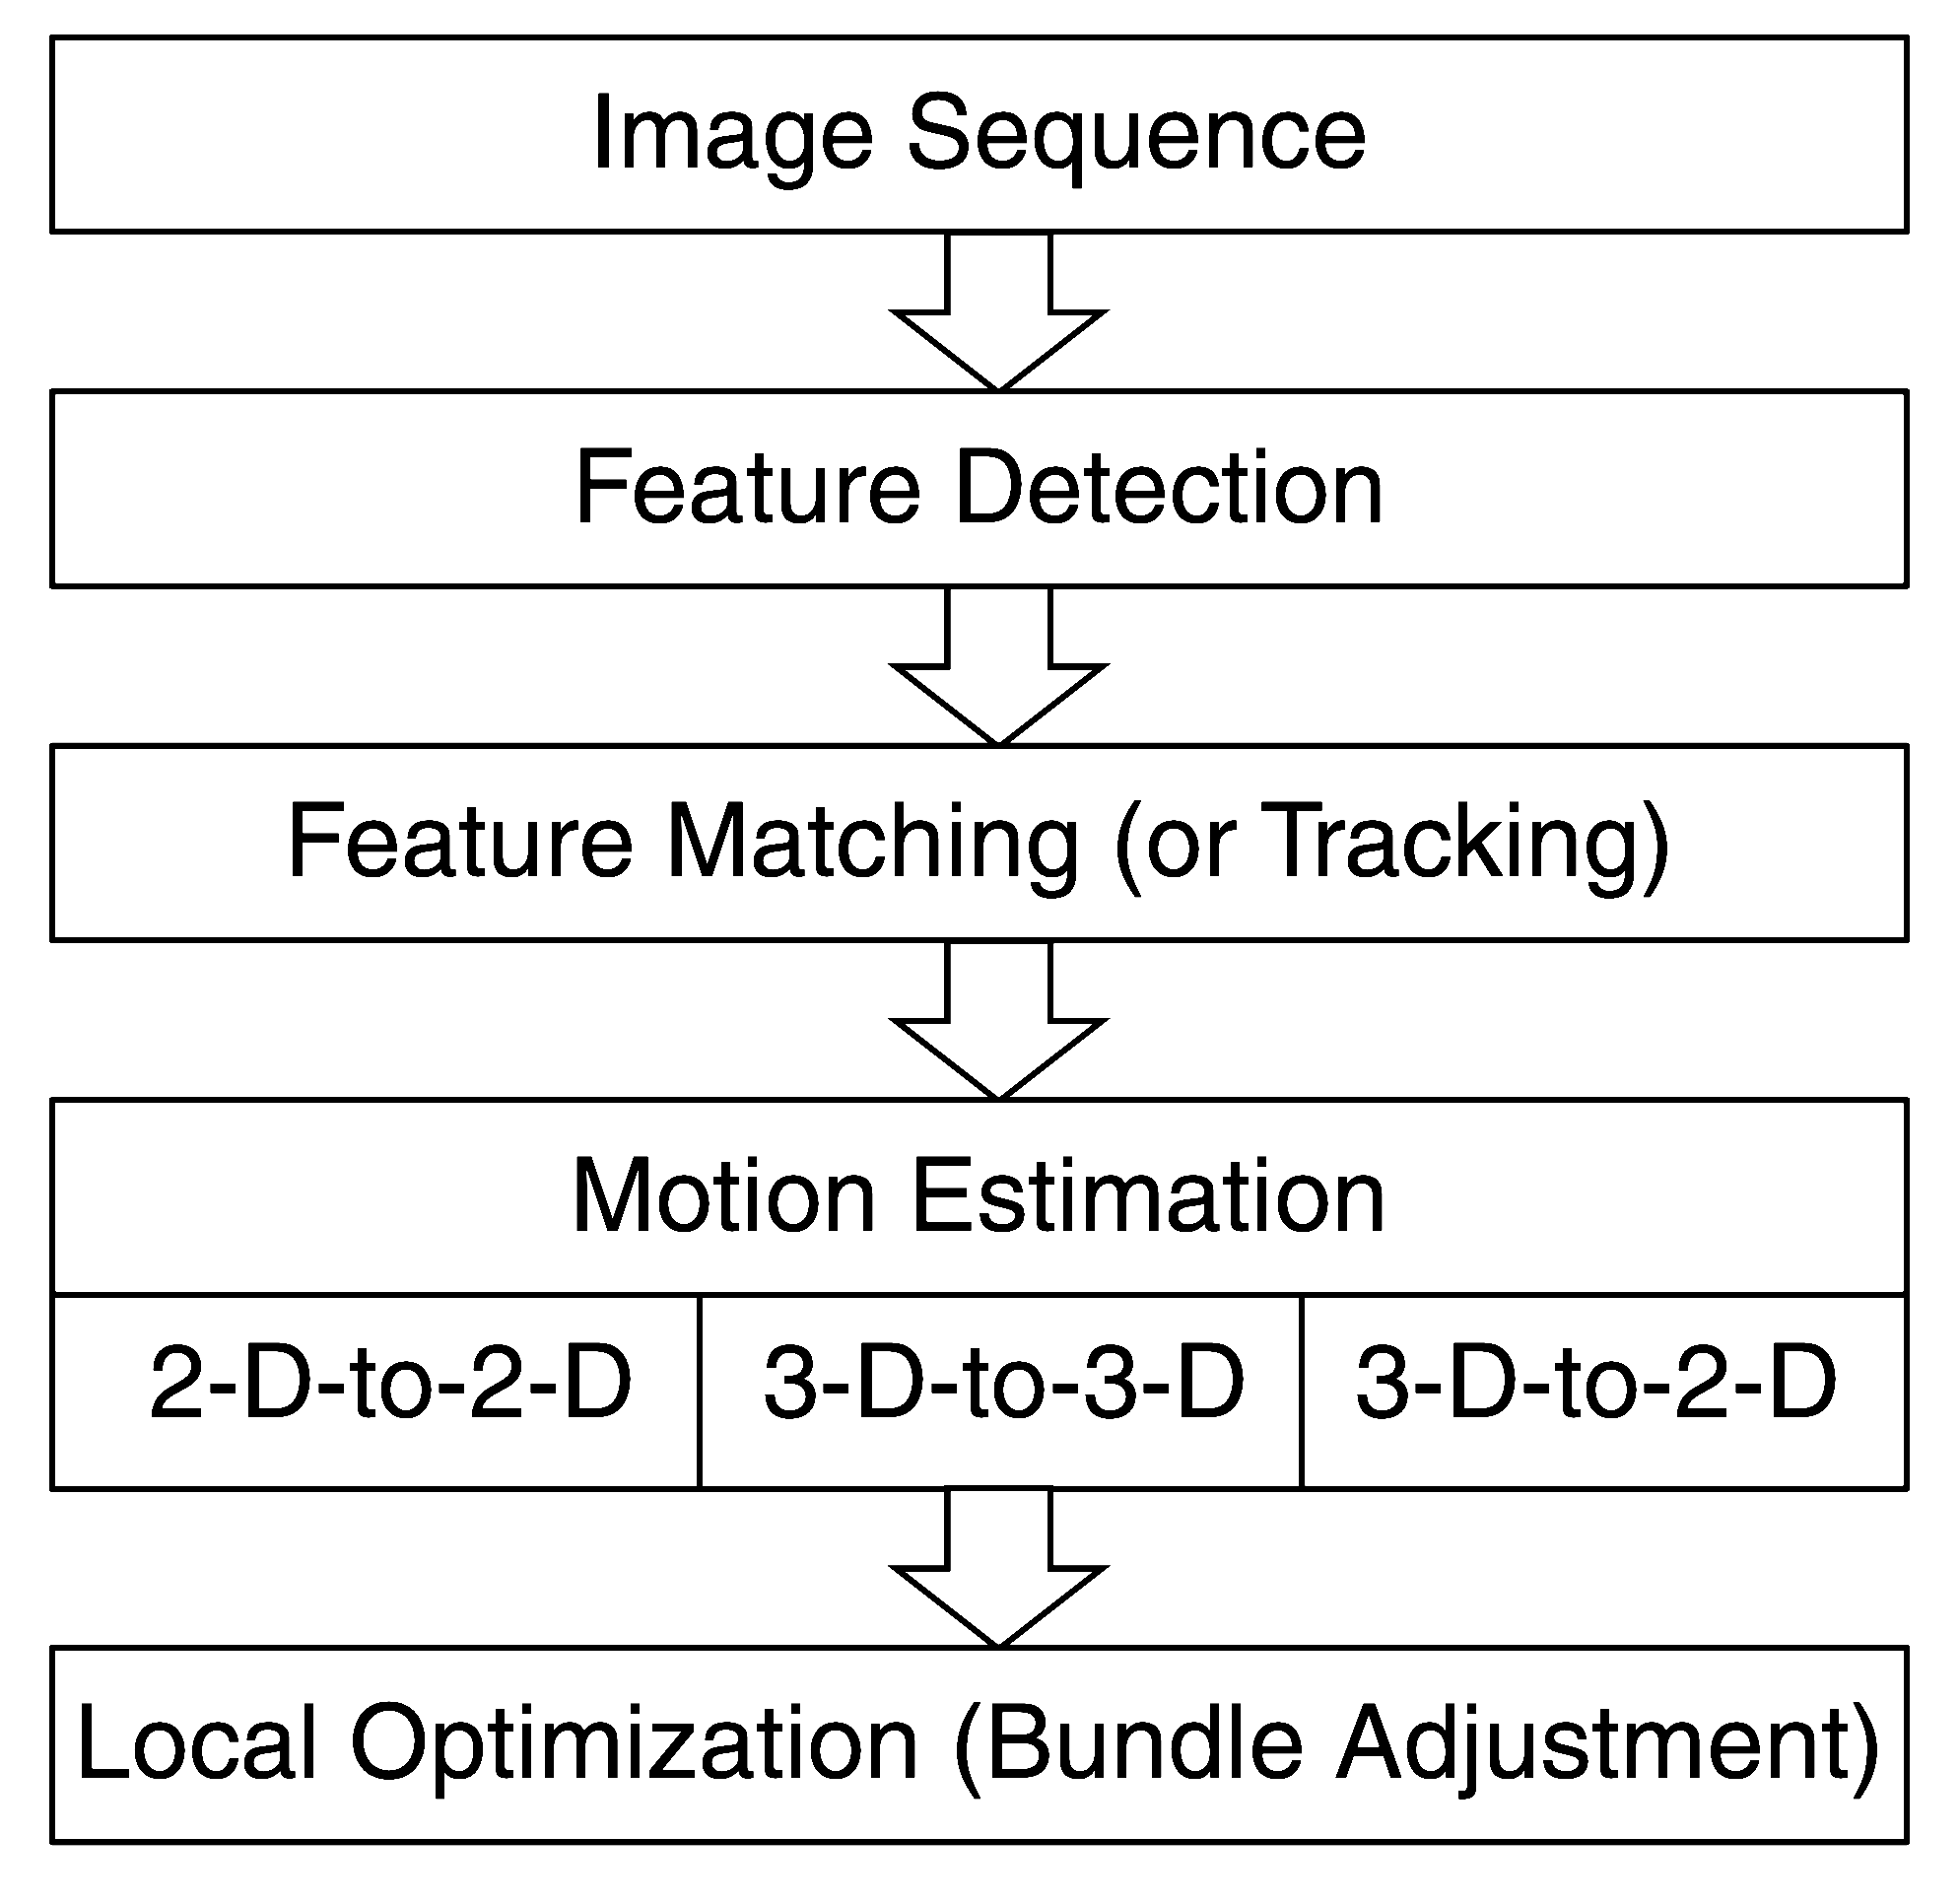
\includegraphics[width=0.45\textwidth]{pictures/vo_pipeline_systementwurf.png}
  \end{center}
  \caption[Visuelle Odometrie Pipeline]{Klassische Pipeline die bei der visuellen Odometrie durchlaufen wird. (In Anlehnung an Scaramuzza, 2011 \cite{ScFrVO})}
\end{figure}
%
%Pipeline
Die Visuelle Odometrie ist ein Verfahren, bei dem die Trajektorie inkrementell geschätzt wird. Der Algorithmus bzw die sog. Visual Odometrie Pipeline wird für jede Schätzung durchlaufen.

\subsection{Merkmalsdetektion}

\begin{figure}[h]
  \begin{center}
    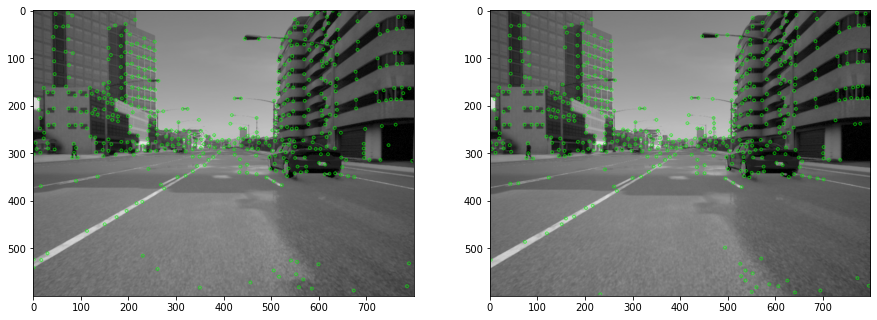
\includegraphics[width=\textwidth]{pictures/feature_detection_systementwurf.png}
    \caption[Merkmalsdetektion in einer CARLA Szene]{Merkmalsdetektion in zwei aufeinanderfolgenden Bildern einer CARLA Szene}
  \end{center}
\end{figure}

Es werden zwei aufeinanderfolgende Bilder $Img_{t-1}$ und $Img_{t+0}$ auf Merkmale untersucht. Die Bilder stammen aus der linken Kamera bei Stereo RGB Setup bzw aus der RGB Kamera beim RGB-D Setup.
\newline

Die Suche nach Merkmalen erfolgt über einen Detektor. Untersucht werden ORB und GFTT. GFTT (Good Features To Track) ist die Implementierung des Shi-Tomasi Interest-Operators und detektiert Kanten im Bild. GFTT ist ein reiner Detektor.

Alternativ wird die Extraktion mittels ORB Detektor betrachtet. Für diesen Fall werden die Merkmale durch einen oriented FAST-9 Detektor gesucht. In anderen Arbeiten wurde gezeigt, dass der ORB Detektor 64 mal schneller Merkmale extrahiert als GFTT, bei gro{\ss}en Veränderungen der Skalierung oder des Kamerawinkels allerdings weniger Merkmale liefert.\cite{Mouats.PerfD}
\newline

Die Detektoren liefern Keypoints für die gefundenen Merkmale. Diese werden an Detektor-Algorithmen übergeben. Ein Detektor ist vergleichbar mit einem Fingerabdruck die eindeutige Beschreibung eines Merkmals. Ein durch einen Detektor beschriebener Keypoint lässt sich auch nach Veränderung im Bild wiederfinden. Diese Robustheit gegenüber Veränderungen wird als Invarianz bezeichnet und ist eine wesentliche Voraussetzung für das MAtching von Merkmalen zwischen zwei Zeitschritten.

Als Deskriptor wird in jedem Fall ORB verwendet.
%
\subsection{Matching von Merkmalen}
% Frame 2 Frame
Beim Matching von Merkmalen wird bestimmt welche Deskriptoren in beiden Bildern auftreten. Durch die Bewegung der Kamera können Merkmale aus der Szene das Bildfeld verlassen bzw hinzugekommen sein. Au{\ss}erdem können Merkmale zB verdeckt  worden sein.\\
Matches sind eine Menge von Deskriptoren, die für beide Bilder $Img_{t-1}$ und $Img_{t+0}$ gültig ist. Durch diese Menge wurde eine Beziehung zwischen den Bildern hergestellt.


Der simpelste Algorithmus für das Matching ist die Implementierung von Brute Force. Als erfolgreiches Match gilt ein Vergleich innerhalb einer Suchregion mit der kleinsten Distanz. Brute Force Matcher liefern gute Ergebnisse, vergleichen allerdings sehr viele Merkmale. Daher ist Brute Force die langsamste Methode für den Abgleich.
\newline

Eine Methode die für gro{\ss}e Mengen an Deskriptoren (>1000) \cite{Mouats.PerfD} schneller sein kann ist der FLANN (Fast Library for Approximate Nearest Neighbors) basierte Matcher. FLANN baut einen KD-Baum und gleicht Deskriptoren nur in einer Nachbarschaft ab. Dadurch werden gute Matches schnell gefunden, das Resultat sind aber nicht zwangsläufig das best-möglichste. Eine Erhöhung der Qualität der Ergebnisse kann über Parameter erfolgen, führt aber zu höheren Kosten in der Laufzeit und erhöht die Gesamtausführungszeit.\\
%
\begin{figure}[!h]
  \begin{center}
    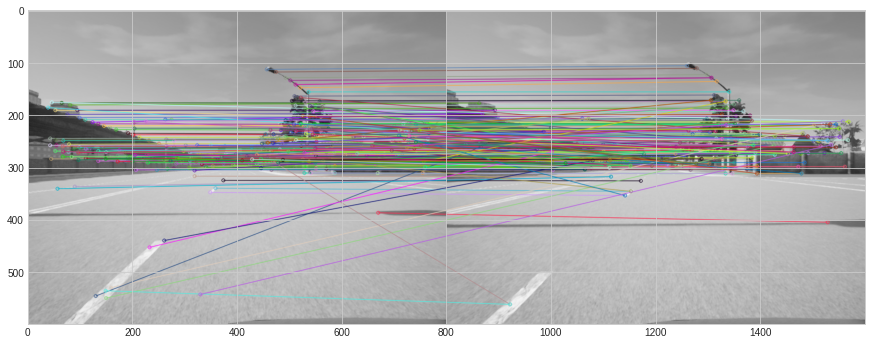
\includegraphics[width=\textwidth]{pictures/bf_matching_no_crosscheck_systementwurf.png}
    \caption[Brute Force Matching ohne Crosscheck]{Brute Force Merkmalsabgleich ohne Cross Checking in zwei aufeinanderfolgenden Bildern einer CARLA Szene.}
  \end{center}
\end{figure}
%
Um ein möglichst robustes Ergebnis zu erzielen wird der Brute Force Matcher mit Cross-Check verwendet. Beim Cross-Check werden die Resultate der beiden Bilder darauf Verglichen, ob das beste Match in Set A auch das beste Match in Set B war und umgekehrt. 
Cross-Checking liefert konsistente Resultate und ist eine Alternative zum sonst verwendeten Lowes Ratio Test für das Filtern von Ausrei{\ss}ern. \cite{cvdocMatch}
%
\begin{figure}[!h]
  \begin{center}
    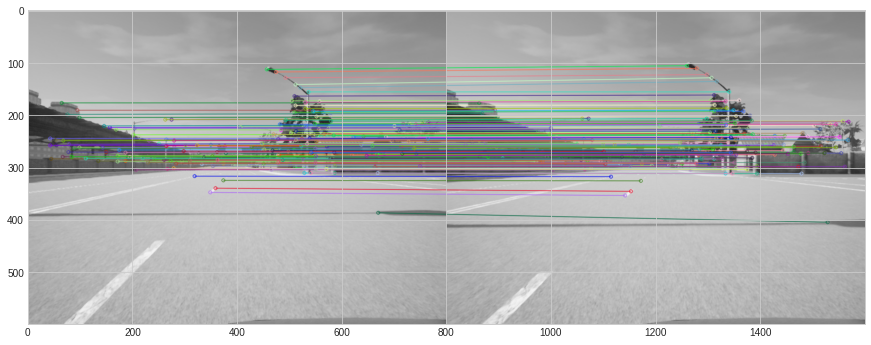
\includegraphics[width=\textwidth]{pictures/bf_matching_with_crosscheck_systementwurf.png}
    \caption[Brute Force Matching mit Crosscheck]{Brute Force Merkmalsabgleich mit Cross Checking in zwei aufeinanderfolgenden Bildern einer CARLA Szene.}
  \end{center}
\end{figure}
%
In der OpenCV Implementierung des Brute Force Matcher kann au{\ss}erdem ebenfalls ein Nachbarschafts-beschränkung mitgegeben werden. Für Binäre Deskriptoren wie ORB wird hier am besten die Hamming Distanz anstatt des Standardmä{\ss}igen Euklidischen Abstands gewählt.


\subsection{Tiefeninformation}
Die zwei simulierten Setups beziehen ihre Tiefeninformation aus unterschiedliche Weise. In jedem Fall kann auf Pixelebene die Tiefe als ein zusätzlicher Kanal betrachtet werden.
%
\begin{figure}[!ht]
  \begin{center}
    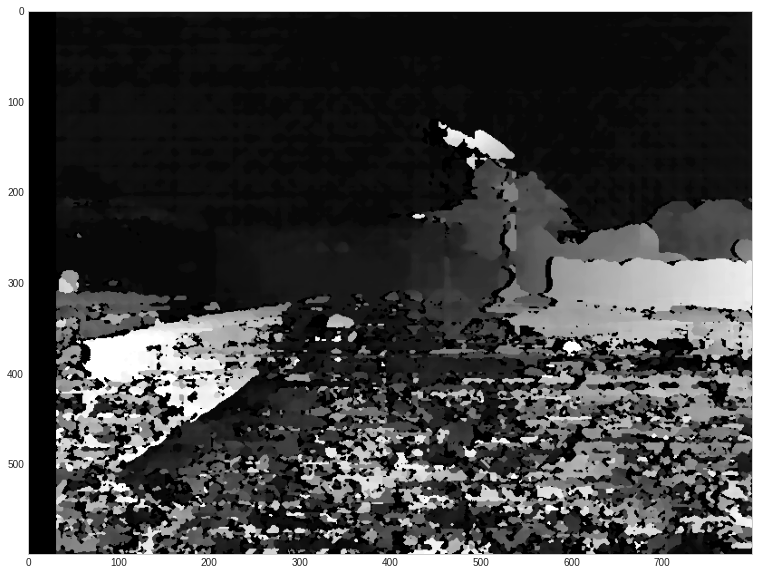
\includegraphics[width=0.5\textwidth]{pictures/disparity_notebook.png}
    \caption[Disparitätenkarte]{Disparitätenkarte als Ergebnis eines Stereo Matchings einer CARLA Szene.}
  \end{center}
\end{figure}
%
Beim Stereo RGB Kamera Setup liegen die Tiefeninformationen nicht direkt vor sondern werden über Triangulation von Stereomatches unter Zuhilfenahme der Epipolargeometrie berechnet.  Daraus entsteht die sog. Disparitätenkarte. Bei der Programmierung wird hier ein StereoMatcher verwendet. StereoMatcher sind Matching Algorithmen die die Epipolaren Beschränkungen gezielt zur Beschleunigung der Suche einsetzen. Im vorgestellten Systementwurf wird ein in OpenCV implementierter Semi-Global Matching Algorithmus basierend auf einem 2008 von Hirschmüller veröffentlichten Paper verwendet. \cite{Hirsch.SGBM}
%

RGB-D liefert das Tiefenbild direkt, weshalb keine zweite Kamera und keine Berechnung der Verschiebung zwischen den Bildern nötig ist. Real wird die Tiefe über eine Time-of-Light Messung bestimmt. In der Simulation werden die Tiefenbilder direkt vom Simulator ausgegeben mit einer maximalen Tiefe von einem Kilometer, was reale ToF Kameras bei weitem übertrifft.

\subsection{Bewegungsschätzung}

Die Bewegungsschätzung erfolgt von Frame zu Frame (F2F). Für jedes Match werden die Pixelkoordinaten aus den Keypoints ausgelesen. Dadurch liegen zwei 2D Punktmengen für die beiden Bilder vor. Für die Matches aus dem vorherigen Bild $Img_{t-1}$ werden au{\ss}erdem die Tiefeninformation der Pixel zu den Punkten hinzugefügt. Die Information lässt sich bei Stereo Kamera aus der Disparitätenkarte lesen bzw aus dem Tiefenbild bei einer RGB-D Kamera.

Dadurch liegen schlie{\ss}lich eine 3D Punktmenge der Matches für $Img_{t-1}$ und ine 2D Punktmenge für $Img_{t+0}$ vor.

Die 3D Punkte aus dem vorherigen Zeitschritt dienen als Objekte im Weltkoordinatensystem zu denen die aktuelle Punkte in Bezug gesetzt werden. Es wird die Transformation gefunden für die der Re-Projektionsfehler am geringsten ist. Die Reprojektion die hier betrachtet wird läuft von den 3D Punkten durch die 2D Bildpunkte zum Kamerabrennpunkt. (Anders als beim Bundle Adjustment wo die Reprojektion auf die 2D Bildpunkte betrachtet wird).


Das Problem des Schätzens der Pose aus Korrespondenzen aus 3D Referenzpunkten und ihrem 2D Abbild in einer kalibrierten Kamera wird als Perspective-from-N-Points Problem (PnP) bezeichnet und ist fundamentaler Bestandteil vieler Computer Vision Anwendungen. Erste Lösungen der Problemstellung existieren bereits seid 1841. Heute wird i.d.R. eine Kombination aus PnP mit RANSAC verwendet, da PnP empfindlich gegenüber Ausrei{\ss}ern ist. RANSAC filtert Ausrei{\ss}er.

Mathematisch wird bei PnP Algorithmen versucht eine eindeutige Lösung für ein überbestimmtes Gleichungssystem aus Polinomgleichungen zu bestimmen. Ohne weitere Information zu den Punkten werden mindestens 4 Punkte für eine eindeutige Lösung benötigt. Die Berechnung für P4P ist jedoch wesentlich komplexer als für $p \geq 5$ weshalb wenn möglich, wie bei der Visuellen Odometrie oder allgemein SLAM Verfahren mit mindestens 5 Punkten berechnet wird.
\newline

Unter Zuhilfenahme des Lochkamera-Modells und der Kameramatrix $K$ werden die 3D Punkte aus der Bildebene (Pixelkoordinaten) in das Kamerakoordinatensystem transformiert.
%
\begin{equation}
\label{eq:sshort}
    sP_{c} = K[R | T]p_{w}
\end{equation}
%
\begin{equation}
  s 
  \begin{bmatrix}u\\v\\1\end{bmatrix} = \begin{bmatrix}
  f_x & \gamma & u_0\\
  0 & f_y & v_0\\
  0 & 0 & 1
  \end{bmatrix}\begin{bmatrix}
  r_{11} & r_{12} & r_{13} & t_{1}\\
  r_{21} & r_{22} & r_{23} & t_{2}\\
  r_{31} & r_{32} & r_{33} & t_{3}\\
  \end{bmatrix}
\begin{bmatrix}x\\y\\z\\1\end{bmatrix}
\end{equation}

Umformung zu 

\begin{equation}
  P_c = K^{-1} \cdot (s \cdot [u, v, 1])
\end{equation}

Bei PnP wird also die Bewegung aus einer 3D zu 2D Transformation geschätzt.

\begin{equation}
\label{eq:tmatrix}
  \begin{split}
T_{k} &= 
    \begin{pmatrix}
    R_{k,k-1} & t_{k,-1}\\
    0 & 1
    \end{pmatrix} \\
    \\
    &= \arg\min_{T_{k}} \sum_{i=1} \left\|p_{k}^i - \hat{p}_{k-1}^i \right\|^2,
  \end{split}
\end{equation}
%

%
\subsection{Pose Update und Verlorene Odometrie}
Ausgabe der Schätzung ist ein Translationsvektor $t$ und eine Rotationsmatrix $R$ für die aktuelle Position. Durch Multiplikation der vorherigen Pose mit $R|t$ wird die aktuelle Pose berechnet. Addition der Posen gibt die Trajektorie.

An dieser Stelle wird ein Update der Output Odometrie vorgenommen und die ROS Transformation von $tf\: \/odom\: \rightarrow\: \/base\_link$. Die ausgegebene Kovarianz wird berechnet durch die Median Absolute Deviation (MAD) zwischen den 3D Merkmalskorrespondenzen.

\begin{equation}
  MAD = median (\|X_i - \tilde{X}_i \|)
\end{equation}

Unter Umständen konnte keine Schätzung durchgeführt werden, Beispielsweise weil nicht genügend Matches gefunden werden konnten. In diesem Fall wird die aktuelle Kameraposition auf die letzte gültige Kameraposition gesetzt.